\documentclass{standalone}
\usepackage{hsbcommon}
%% Show/hide steps for standalone work — edit this line:
\makeatletter\AtBeginDocument{\@buildstepset{1,2,3,4}}\makeatother
\begin{document}
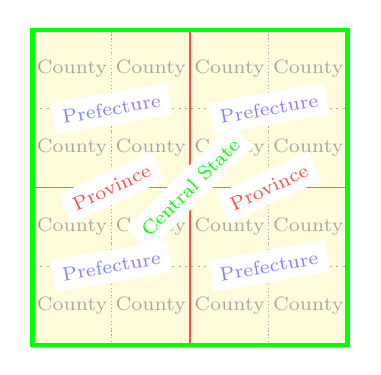
\begin{tikzpicture}
    \tikzset{
        mycounty/.style={draw}
    }

    \filldraw[yellow!40] (1,1) rectangle (5,5);

    \ifstep{1,county}{
    \begin{scope}
    \foreach [count=\i] \mya in {1,...,4}
        \foreach [count=\ii] \myb in {1,...,4}
            \draw[dotted] (\i,\ii) rectangle node {\scriptsize County} (\i+1,\ii+1);
    \end{scope}
    }

    \ifstep{2,prefecture}{
    \begin{scope}[blue]
    \filldraw[white,opacity=0.3] (1,1) rectangle (5,5);
    \foreach[count=\i] \mya in {1,3}
        \foreach[count=\i] \myb in {1,3}
            \draw (\mya,\myb) rectangle node[fill=white,rotate=10,opacity=1] {\scriptsize Prefecture} (\mya+2,\myb+2);
    \end{scope}
    }

    \ifstep{3,province}{
    \begin{scope}[red]
    \filldraw[white,opacity=0.3] (1,1) rectangle (5,5);
    \foreach[count=\i] \mya in {1,3}
            \draw[thick] (\mya,1) rectangle node[fill=white,rotate=25] {\scriptsize Province} (\mya+2,5);
    \end{scope}
    }

    \ifstep{4,central}{
    \begin{scope}[green]
    \filldraw[white,opacity=0.3] (1,1) rectangle (5,5);
        \draw[ultra thick] (1,1) rectangle node[fill=white,rotate=45] {\scriptsize Central State} (5,5);
    \end{scope}
    }
        

\end{tikzpicture}
\end{document}